\chapter{Required Properties of E2E Systems\ifdraft{ (Dan) (35\%)}{}}
\label{chapter:required_properties}

We now describe the required properties that E2E VIV systems must have
in order to be considered for use in real elections. These
requirements can be broadly divided into two groups: \emph{technical
  requirements} and \emph{non-functional requirements}. Technical
requirements are those that can be directly addressed by the design
and implementation of the system, such as authentication requirements
for voters and election officials. Non-functional requirements are
those that are imposed on the system by external entities or where the
system depends on external behaviors outside its control, such as
specific election certification guidelines and operational
procedures. Each of these groups is itself divided into several
categories, and \autoref{fig:e2eviv_requirements_hierarchy} gives a
high-level overview of these.

\begin{figure}
\begin{center}
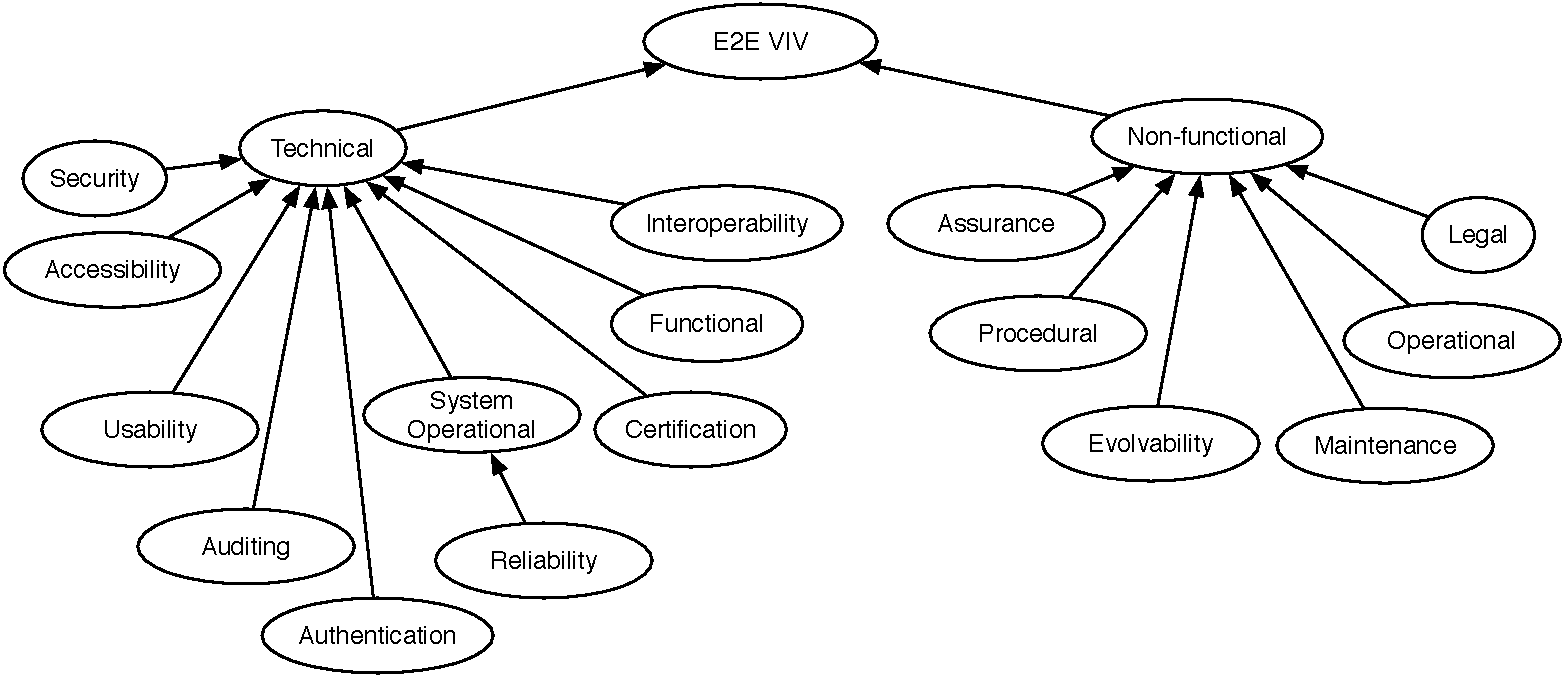
\includegraphics[width=6in]{required_properties_resources/hierarchy}
\end{center}
\caption{The hierarchy of requirements for E2E VIV systems.}
\label{fig:e2eviv_requirements_hierarchy}
\end{figure}

The following is a high-level description of the categories and the
requirements within each; \autoref{appendix:bon_requirements} is a
complete listing of the requirements expressed in the Business Object
Notation.\tododmz{is \autoref{appendix:bon_requirements} actually
  necessary, or will everything basically be described here?}

\section{Technical Requirements}
There are ten categories of technical requirements for E2E VIV
systems: functional, accessibility, usability, security,
authentication, auditing, system operational, reliability,
certification, and interoperability.

\subsection{Functional} 
\todogeneric{Should this really be ``functional''? Would ``core'' or
  something similar work better? It seems that some other
  requirements, such as those dealing with auditing and counting, are
  also functional...}  The functional requirements of an E2E VIV
system deal primarily with the casting and recording of ballots and
associated voter records. One important requirement is that there must
be a correspondence between the recorded ballots and the voters that
are listed as having voted; a ballot cannot be recorded without a
voter casting it, and a voter cannot be listed as having voted without
casting a ballot. Similarly, if a voter is informed by the system that
her ballot has been successfully cast, the system must correctly
retain the record of her having voted and her cast ballot information
even in the event of server failures.

Another functional requirement is the property of \emph{receipt
  freedom}: it must be impossible for a voter to prove to anybody any
information regarding how they voted their ballot, beyond what can be
mathematically deduced from the final distribution of votes. For
example, if a referendum passes with 100\% of the vote, there is no
way to hide the fact that every voter approved of the referendum;
however, if the result is mixed, it must be impossible for any
individual voter to prove how they voted.

In some elections voters are allowed to cast multiple ballots with
only the last cast ballot counting toward the final election tally,
while in others voters are prohibited from casting multiple
ballots. The system must accommodate both of these election formats,
ensuring that only the last cast ballot is counted for each voter when
multiple ballots are allowed and ensuring that each voter casts at
most one ballot otherwise.

Maintaining voter anonymity is critical, so it must be impossible
after the election to reconstruct a link between a cast ballot and any
identifying information about the voter who cast it. However, in
systems that support the casting of multiple ballots, it is important
to maintain links between voters and their ballots \emph{during} the
election to ensure that later ballots replace the correct earlier
ballots. To balance these concerns, it is a functional requirement of
the system that once it is determined that a ballot will be counted
toward the final tally, any link between that ballot and the voter who
cast it must be irrevocably broken.

Finally, because the voter should be able to focus on the voting
process without undue distractions or external influences, the voting
system must not display or permit the display of any advertising or
commercial logos during a voting session; the exception to this rule
is that an election jurisdiction may display its own logo to the voter
during the voting process. Along the same lines, the voting system
must not display any links to other Internet sites outside of the
voting system, except to provide help with the actual mechanics of
voting.

\subsection{Usability}

The usability of an E2E VIV system is critical to its successful
adoption and use. Since the user experience is so important, many of
the requirements of the system have some relation to usability even
though they may be categorized under other headings. There are,
however, two requirements that are exclusively related to the
usability of the system with respect to vote casting and one general
usability requirement that applies to the system as a whole.

The first vote casting requirement is that, if a voter receives a
final vote confirmation (e.g., ``Thank you for voting!'' or a similar
notice) from the system, she can be certain that her ballot was
recorded correctly. This is the usability counterpart to the
functional requirement that ballot records and voter records must be
maintained correctly even in the event of server failures.

The second vote casting requirement is that, if a voter is uncertain
whether or not her ballot was recorded (e.g., she clicked a ``submit''
button but never got a response from the system), she must be free
to attempt to vote again.

Finally, usability testing must be performed on any E2E VIV system
before it is deployed. The reports of the usability testing must be
made public, and the system must achieve satisfactory test results
before being used in a binding election.


\subsection{Accessibility}

Accessibility---the property of being usable by and useful to the
disabled---is one of the main goals of an E2E VIV system. It is
closely related to usability, but there are several requirements
associated specifically with accessibility that go beyond typical
usability requirements. 

Users must be involved in the design of the system to identify
accessibility constraints at each stage of the development
process. Consideration must be given to the system's compatibility
with existing technologies designed to help disabled individuals; for
example, the system should be developed in a way that allows assistive
input devices such as switches and eye trackers to be used in addition
to keyboards, mice and touchscreens. Similarly, the system's
presentation of voting options should be optimized to voters' needs by
providing alternative display fonts, audio representations, braille
representations, and other representations as appropriate.

All possible measures must be taken to ensure that the system can be
used by all voters and, if that is not possible in all circumstances,
to provide access to alternative methods of voting for those voters
who cannot use the system.

Finally, accessibility testing must be performed in addition to the
previously-mentioned mandatory usability testing. The reports of the
accessibility testing must be made public, and the system must achieve
satisfactory test results before being used in a binding election.

\subsection{Security}

Security is the largest category of technical requirements, comprised
both of requirements on the security and integrity of the system
infrastructure (data storage, communications, etc.) and of
requirements on the security and integrity of the voting process
(voter authorization, voter privacy, accuracy of the final tally,
etc.).

With respect to the system infrastructure, it is critical that data
integrity be ensured throughout the system. This means that measures
must be taken to ensure that no data can be permanently lost in the
event of a breakdown or fault affecting the system; that the system
must maintain the integrity of the voters' register, lists of
candidates, ballot information, cast ballots, and other critical
information, in addition to authenticating the original source(s) of
that information and tracking provenance where appropriate; that all
data communications within the system must have associated integrity
checks; that system equipment under the control of the electoral
authority must be protected against influences that could modify the
election results; and that the integrity of the election results must
not depend in any way upon the security of system equipment not under
control of the electoral authority.


\subsection{Authentication}
\lipsum[6]
\subsection{Auditing}
\lipsum[7]
\subsection{System Operational}
\lipsum[8]
\subsection{Reliability}
\lipsum[9]
\subsection{Certification}
\lipsum[10]
\subsection{Interoperability}
\lipsum[11]

\section{Non-functional Requirements}
There are six categories of non-functional requirements for E2E VIV
systems: operational, procedural, legal, assurance, maintenance, and
evolvability.

\subsection{Operational}
\lipsum[13]

\subsection{Procedural}
\lipsum[14]

\subsection{Legal}
\lipsum[15]

\subsection{Assurance}
\lipsum[16]

\subsection{Maintenance}
\lipsum[17]

\subsection{Evolvability}
\lipsum[18]
